\documentclass[a4paper,12pt]{article}
%%%%%%%%%%%%%%%%%%%%%%%%%%%%%%%%%%%%%%%%%%%%%%%%%%%%%%%%%%%%%%%%%%%%%%%%%%%%%%%%%%%%%%%%%%%%%%%%%%%%%%%%%%%%%%%%%%%%%%%%%%%%%%%%%%%%%%%%%%%%%%%%%%%%%%%%%%%%%%%%%%%%%%%%%%%%%%%%%%%%%%%%%%%%%%%%%%%%%%%%%%%%%%%%%%%%%%%%%%%%%%%%%%%%%%%%%%%%%%%%%%%%%%%%%%%%
\usepackage{eurosym}
\usepackage{vmargin}
\usepackage{amsmath}
\usepackage{graphics}
\usepackage{epsfig}
\usepackage{framed}
\usepackage{subfigure}
\usepackage{fancyhdr}

\setcounter{MaxMatrixCols}{10}
%TCIDATA{OutputFilter=LATEX.DLL}
%TCIDATA{Version=5.00.0.2570}
%TCIDATA{<META NAME="SaveForMode"CONTENT="1">}
%TCIDATA{LastRevised=Wednesday, February 23, 201113:24:34}
%TCIDATA{<META NAME="GraphicsSave" CONTENT="32">}
%TCIDATA{Language=American English}

\pagestyle{fancy}
\setmarginsrb{20mm}{0mm}{20mm}{25mm}{12mm}{11mm}{0mm}{11mm}
\lhead{Advanced Data Modelling} \rhead{Logistic Regression} \chead{MA4128} %\input{tcilatex}

%http://www.electronics.dit.ie/staff/ysemenova/Opto2/CO_IntroLab.pdf
\begin{document}
\begin{framed}
\noindent \textbf{What are odds?}\\
The odds of outcome 1 versus outcome 2 are the probability (or frequency) of outcome 1 divided by the probability (or frequency) of outcome 2.
\end{framed}
	\section*{Question 1: Odds Example}
	There are 5 pink marbles, 2 blue marbles, and 8 purple marbles.
	
	\begin{itemize}
		\item What is the probability of picking a blue marble? (Answer: 2/15).
		\item What are the odds in favor of picking a blue marble? (Answer: 2/13).
	\end{itemize}

	\section*{Question 2: Odds Ratio Example}

Suppose that seven out of 10 males are admitted to an engineering school while three of 10 females are admitted. 

\begin{itemize}
	\item The probabilities for admitting a male are,
	p = 7/10 = 0.7      ( q = 1 - 0.7 = 0.3)
	\item Here are the same probabilities for females,
	p = 3/10 = 0.3       (q = 1 - 0.3 = 0.7)
\end{itemize}
Now we can use the probabilities to compute the admission odds for both males and females,
\begin{itemize}
	\item \textit{odds(male) }= 0.7/0.3 = 2.33333
	\item \textit{odds(female) }= 0.3/0.7 = 0.42857
\end{itemize}
Next, we compute the odds ratio for admission,
\[OR = 2.3333/0.42857 = 5.44\]
Thus, for a male, the odds of being admitted are 5.44 times as large than the odds for a female being admitted.

\section*{Question 3: Odds Ratio Example}
	\begin{itemize}
		\item Suppose that in a sample of 100 men, 90 drank wine in the previous week, while in a sample of 100 women only 20 drank wine in the same period. \item The odds of a man drinking wine are 90 to 10, or 9:1, while the odds of a woman drinking wine are only 20 to 80, or 1:4 = 0.25:1. 
		\item The odds ratio is thus 9/0.25, or 36, showing that men are much more likely to drink wine than women. 
		\item The detailed calculation is:
		
		
		\[ { 0.9/0.1 \over 0.2/0.8}=\frac{\;0.9\times 0.8\;}{\;0.1\times 0.2\;} ={0.72 \over 0.02} = 36 \]
		
		\item This example also shows how odds ratios are sometimes sensitive in stating relative positions: in this sample men are 90/20 = 4.5 times more likely to have drunk wine than women, but have 36 times the odds. 
		
		
		
		\item The logarithm of the odds ratio, the difference of the logits of the probabilities, tempers this effect, and also makes the measure symmetric with respect to the ordering of groups. 
		\item For example, using natural logarithms, an odds ratio of 36/1 maps to 3.584, and an odds ratio of 1/36 maps to -3.584.
	\end{itemize}

	
\section*{Question 4: Odds Ratio Example}
	These data are taken from the British Election Study 2005 pre-campaign and
	post-election panel data. We will consider the propensity to vote (sometimes called ‘turnout’) as the
	dependent variable, which has 2 categories. 
	out to vote.
	\begin{center}
		\begin{figure}[h!]
			% Requires \usepackage{graphicx}
			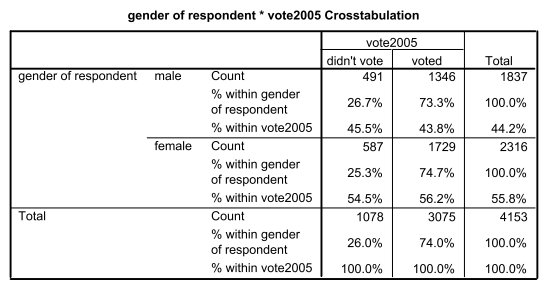
\includegraphics[scale=0.8]{LogWeek10A}\\
		\end{figure}
	\end{center}
\begin{itemize}
	\item The odds of a male turning out to vote are:
	\[1346/491 = 2.741\]
	\item The odds of female turning out to vote are
	\[1729/587 = 2.945\]
	\item The Odds ratio (female: male) are
	\[ \frac{1729/587 }{ 1346/491 } = \frac{2.945}{2.741}= 1.074\]
\end{itemize}	

\begin{framed}
\noindent \textbf{The Logit}\\
\begin{itemize}
	\item 		The convention for binomial logistic regression is to code the
	dependent class of greatest interest as 1 and the other class as 0, because the coding will
	affect the odds ratios and slope estimates.
	
\item 	The logit(p) is the log (to base e) of the odds ratio or likelihood ratio that the dependent
	variable is 1. In symbols it is defined as:
	\[ logit(p) = ln \left(\frac{p}{(1-p)}\right) \]
	
\item	Whereas p can only range from 0 to 1, logit(p) scale ranges from negative infinity to positive
	infinity and is symmetrical around the logit of 0.5 (which is zero)
\end{itemize}

\end{framed}
	%---------------------------%
\section*{Question 5: Logistic Transformation}
\begin{itemize}
	\item 
	Given that $p_i = 0.2$, compute $\eta_i$.
	
	\[ \eta_i = \log \left( \frac{0.2}{1-0.2} \right)= \log\left( \frac{0.2}{0.8} \right)\] 
	
	\[ \eta_i =  \mbox{log}(0.25) =-1.386 \]
	
\item Given that $\eta_i = 2.3$, compute $p_i$.
	\[ \pi_i  =  \frac{e^{2.3}}{1 + e^{2.3}} = \frac{9.974}{1 + 9.974} = 0.908 \]
\end{itemize}
\section*{Question 6: Classification}
	Let us suppose that the probability of survival of a marine species of fauna is dependent on pollution, depth and water temperature. Suppose the logit for the logistic regression was computed as follows:
	\[ \eta_i = 0.14 + 0.76x_1 - 0.093x_2 + 1.2x_3  \]
	\begin{center}
		\begin{tabular}{|c|c|c|}
			\hline
			% after \\: \hline or \cline{col1-col2} \cline{col3-col4} ...
			Variables & case 1 & case 2 \\ \hline
			Pollution($x_1$) & 6.0 & 1.9 \\
			Depth ($x_2$)& 51 & 99 \\
			Temp ($x_3$) & 3.0 & 2.9 \\
			\hline
		\end{tabular}
	\end{center}
	Compute the probability of success for both case 1 and case 2.
	
	\begin{itemize}
		\item case 1$ \eta_1 = 0.14 + (0.76 \times 6)	- (0.093\times 51) + (1.2\times 3) = 3.557$
		\item case 2$ \eta_2 = 0.14 + (0.76 \times 1.9)	- (0.093\times 99) + (1.2\times 2.9) = -4.143$
	\end{itemize}
	
	The probabilities for success are therefore:
	\[ \pi_1  =  \frac{e^{3.557}}{1 + e^{3.557}} = \frac{35.057}{1 + 35.057} = 0.972 \]
	\[ \pi_2  =  \frac{e^{-4.143}}{1 + e^{-4.143}} = \frac{0.0158}{1 + 0.0158} = 0.0156 \]
	
		%--------------------------------------------------------%
\section*{Question 7: Wald Test}
\noindent
For the logistic regression model described in the SPSS output below, state the Odds Ratio for each variable. State the 95\% confidence interval for the Odds Ratio in each case. Comment on this significance of each predictor variable.
		\begin{figure}[h!]
			\centering
			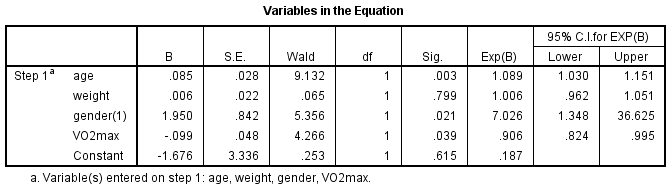
\includegraphics[width=0.9\linewidth]{images/waldtest}

		\end{figure}

\end{document}